% Статья для Physical Review E, основная (русская) версия; английский текст ждёт обновления в main_en.tex. Сборка: pdflatex, bibtex, pdflatex, pdflatex в этой папке;
% рисунки читают данные моделирования из родительской папки. Рис. 1(a): LANG=ru python3 fig_array.py -> fig_array_ru.pdf.
\documentclass[pre,twocolumn,superscriptaddress,showpacs=false,amsmath,amssymb,nofootinbib]{revtex4-2}
\usepackage[T2A]{fontenc}
\usepackage[utf8]{inputenc}
\usepackage[english,russian]{babel}

\usepackage{pgfplots}
\pgfplotsset{compat=1.18}
\usepackage[unicode,colorlinks=true,linkcolor=blue!50!black,citecolor=blue!50!black,urlcolor=blue!50!black]{hyperref}
\usepackage{microtype}
\newcommand{\datadir}{..}

\begin{document}

\title{Встряска после промаха, покой после попадания: диффузия, зависящая от исхода, и обучение нейронов в культуре, играющих в понг}

\author{Константин Кладко}
\email{stan.kladko@skale.network}
\affiliation{SKALE Foundation, 1160 Battery Street East, San Francisco, CA 94111, USA}

\begin{abstract}
Система, параметры которой получают случайные толчки с дисперсией $\sigma_m^2$ после неудачи и $\sigma_h^2$ после успеха, диффундирует с коэффициентом, зависящим от состояния, $D\propto\kappa+(1-\kappa)P$, где $P$~--- локальная вероятность неудачи, а $\kappa=\sigma_h^2/\sigma_m^2$. При шагах, размер которых задаётся в точке отправления (соглашение Ито), стационарная плотность есть $\rho\propto1/D$: неудачи становятся реже случайного уровня при $\kappa<1$, не меняются при $\kappa=1$ и учащаются при $\kappa>1$. В форме оператора Шрёдингера в мнимом времени динамика имеет основное состояние $\phi_0\propto D^{-1/2}$ с нулевой энергией и щель $\propto\sigma_m^2$, так что сила толчков задаёт скорость обучения, но не его конечный уровень; стационарное состояние~--- закон Больцмана с потенциалом $\ln D$ при единичной температуре, понизить которую могут лишь толчки, растущие вместе с $P$. Мы проверяем это на DishBrain, где культуры корковых нейронов играют в понг, а промах вызывает стимуляцию вдвое большей амплитуды, чем стимул после попадания, и паузу в 8~с. В опубликованных данных внутри сеанса улучшается только условие «Стимул» ($+0{,}152$ отбитых мяча за розыгрыш, $p=0{,}0002$; «Тишина» $-0{,}03$ и «Без обратной связи» $-0{,}002$, незначимо), и все условия заканчивают на одном уровне ($p=0{,}22$), как и предсказывает масштабирование щели; уровни покоя различаются между группами ($p=7\times10^{-5}$). Импульсная сеть, откалиброванная по статистике записей покоя, не содержит сенсомоторного пути ни при какой плотности от 375 до $1{,}2\times10^5$ нейронов на мм$^2$ ($10^6$ нейронов): импульсы лишь подавляют моторные области, со слабым смещением «вверх--вниз», которое уводило бы ракетку от мяча. Поэтому она не может показать обучение в замкнутом контуре, но её эмерджентное $\kappa$ при локальной пластичности равно 0{,}6--0{,}8 при околопороговом вовлечении и превышает 1 при широком, и задаётся паузой, а не амплитудой импульсов. Одинаковая пауза после попаданий и промахов разделяет эти две возможности.
\end{abstract}

\maketitle

\section{Введение}

Случайный поиск, прерываемый успехом,~--- один из старейших механизмов обучения: ультраустойчивый гомеостат Эшби меняет параметры наугад, пока его существенные переменные не вернутся в допустимые пределы \cite{Ashby1952}; конечные автоматы, меняющие состояние только при штрафе, ведут себя лучше случайного \cite{Tsetlin1961,Tsetlin1963,Robbins1952}; мокрицы собираются в сырых местах, потому что в сухом воздухе двигаются больше \cite{Gunn1937}. На языке физики это случайные блуждания с шагом, зависящим от положения, а такие блуждающие частицы скапливаются там, где движутся медленно \cite{Schnitzer1993,vanKampen1988,Landauer1988}. Насколько сильно они скапливаются и в каком соглашении читать мультипликативный шум~--- классические вопросы стохастической динамики \cite{Volpe2016}.

Здесь положение~--- это конфигурация обучающейся сети, а размер шага зависит от того, как она играет. Экспериментальный повод~--- DishBrain \cite{Kagan2022}: культуры корковых нейронов на многоэлектродной матрице высокой плотности играют в понг (рис.~\ref{fig:dish}). Спайки в четырёх моторных областях двигают ракетку, а положение мяча подаётся на восемь сенсорных электродов. После попадания культура получает «предсказуемый» стимул (100~Гц в течение 100~мс на всех восьми электродах при 75~мВ); после промаха~--- «непредсказуемый» (150~мВ при 5~Гц в случайных точках и в случайные моменты в течение 4~с), за которым следуют 4~с без стимуляции и новая подача. Культуры улучшали игру в течение сеанса, и это было прочитано как свидетельство того, что нейроны действуют так, чтобы сделать свой вход предсказуемым, как предлагает принцип свободной энергии \cite{Friston2010,Kagan2022}. Однако амплитуда 150~мВ была выбрана, чтобы вызывать потенциалы действия «независимо от состояния клетки, тем самым сильнее возмущая культуру» \cite{Kagan2022}: обратная связь после промаха одновременно менее предсказуема и более разрушительна, и опубликованные контроли не разделяют эти два свойства. Прежняя критика касалась терминов «интеллект» и «чувствительность» \cite{Balci2023,Kagan2023reply}; более близкие прецеденты в культурах~--- принцип регуляции стимула \cite{Shahaf2001,Marom2002} и обучение избеганием стимуляции \cite{Sinapayen2017,Masumori2020}.

\begin{figure*}[t]
\centering
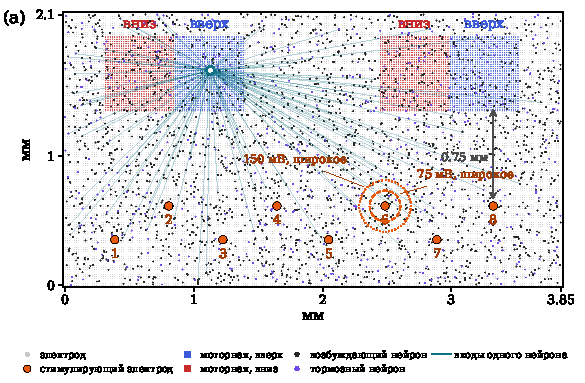
\includegraphics[width=0.56\textwidth]{fig_array_ru.pdf}\hfill
\begin{tikzpicture}[x=1.1cm,y=1.1cm,font=\scriptsize]
\node[font=\small,anchor=south west,inner sep=0] at (-1.35,3.3) {(b)};
\node[anchor=south,align=center,blue!70!black,inner sep=2pt] at (1.3,2.62) {каждые 10 мс спайки областей «вверх» минус «вниз»\\(каждая нормирована на бегущее среднее 20 Гц) двигают ракетку};
\draw[thick] (0,0) rectangle (2.6,2.6);
\foreach \i in {1,...,7}{\draw[orange!50!black,dotted] (2.42,{\i*0.325}) -- (2.6,{\i*0.325});}
\foreach \i in {0,...,7}{\pgfmathtruncatemacro{\k}{\i+1}\node[orange!50!black,anchor=west,inner sep=1pt] at (2.64,{0.1625+\i*0.325}) {\k};}
\draw[line width=3pt,blue!70!black] (2.6,1.04) -- (2.6,1.56);
\node[blue!70!black,anchor=east,inner sep=2pt] at (2.52,1.3) {ракетка $p$};
\fill (0.9,1.95) circle (0.055); \draw[-latex] (0.9,1.95) -- (1.45,1.72);
\draw[orange!50!black,dashed] (0.9,1.95) -- (2.6,1.95);
\node[anchor=south west,inner sep=1pt] at (0.95,2.0) {мяч $(x,y)$};
\draw[-latex,orange!50!black] (0.15,-0.2) -- (2.45,-0.2);
\node[orange!50!black,anchor=north,align=center,inner sep=2pt] at (1.3,-0.25) {код частоты: 4 имп./с у дальней стенки, 40 у стенки ракетки\\код места: электрод $k=\lfloor8(y-p+\tfrac12)\rfloor$, метки справа};
\end{tikzpicture}

\vspace{8pt}
\begin{tikzpicture}[x=0.78cm,y=1cm,font=\scriptsize]
\node[font=\small,anchor=south west,inner sep=0] at (-3.6,2.85) {(c)};
\node[anchor=east] at (-0.2,2.55) {после попадания};
\fill[red!70!black] (0,2.4) rectangle (0.12,2.7);
\node[anchor=west] at (0.2,2.55) {75 мВ, 100 имп./с, 100 мс, все восемь электродов сразу («Тишина»: 100 мс тишины)};
\node[anchor=east] at (-0.2,1.75) {«Стимул», после промаха};
\draw[red!70!black] (0,1.75) -- (4,1.75);
\foreach \t in {0.13,0.41,0.55,0.9,1.27,1.5,1.83,2.1,2.4,2.62,2.95,3.2,3.44,3.7,3.88}{\draw[red!70!black,line width=1.2pt] (\t,1.6)--(\t,1.9);}
\node[anchor=north,red!70!black] at (2,1.56) {150 мВ, 5 имп./с, случайные электроды и моменты, 4 с};
\draw[gray,dashed] (4,1.6) rectangle (8,1.9); \node[gray!40!black] at (6,1.75) {без стимуляции, 4 с};
\node[anchor=west] at (8.05,1.75) {новая подача};
\node[anchor=east] at (-0.2,0.85) {«Тишина», после промаха};
\draw[gray,dashed] (0,0.7) rectangle (8,1.0); \node[gray!40!black] at (4,0.85) {без стимуляции, 8 с};
\node[anchor=west] at (8.05,0.85) {новая подача};
\node[anchor=east] at (-0.2,0.15) {«Без обратной связи», после промаха};
\draw[orange!50!black,thick] (0,0.15) -- (8.4,0.15);
\node[anchor=north,orange!50!black] at (4.2,0.1) {мяч отскакивает от стенки, игра продолжается; коды места и частоты не прерываются};
\draw[-latex] (0,-0.62) -- (8.8,-0.62); \foreach \t in {0,2,4,6,8}{\draw (\t,-0.57)--(\t,-0.67); \node[anchor=north] at (\t,-0.68) {\t};} \node[anchor=north] at (8.85,-0.68) {с};
\end{tikzpicture}
\caption{DishBrain, как он смоделирован. (a) Матрица в масштабе, какой её видит сетевая модель: все 26\,400 электродов сетки $220\times120$ (шаг 17{,}5~мкм), восемь стимулирующих электродов сенсорной полосы зигзагом, как на рис.~4D работы \cite{Kagan2022}, четыре моторные области по $31\times33$ электрода, уравновешенные «вверх» и «вниз», широкие радиусы вовлечения импульсов 75 и 150~мВ (0{,}12 и 0{,}20~мм) вокруг электрода 6, одна реализация 3000 нейронов (80\% возбуждающих) и 100 входов одного нейрона области «вверх», выбранных с вероятностью $\propto e^{-d/\lambda}$, $\lambda=1$~мм: их медианное расстояние 1{,}0~мм, и 10 из них лежат ближе 0{,}2~мм к стимулирующему электроду. (b) Игра: высота мяча относительно ракетки выбирает электрод (код места), а расстояние до стенки ракетки задаёт частоту импульсов (код частоты); каждые 10~мс число спайков в областях «вверх» и «вниз», нормированное на бегущее усиление 20~Гц, двигает ракетку. (c) Обратная связь после каждого исхода в трёх условиях. В сеансах покоя игра идёт вовсе без стимуляции. Напряжения, частоты, длительности и расположение электродов взяты из работы \cite{Kagan2022}; размер поля, полудлина ракетки и скорость мяча~--- выбор модели (приложение~\ref{app:net}).}
\label{fig:dish}
\end{figure*}

Мы формулируем обучение возмущением, зависящим от исхода, как диффузию без сноса с коэффициентом диффузии, зависящим от исхода (разд.~\ref{sec:model}), точно решаем её стационарное состояние и релаксацию (разд.~\ref{sec:results}) и проверяем предсказания на опубликованных данных (разд.~\ref{sec:data}) и на импульсной сети, откалиброванной по культурам (разд.~\ref{sec:net}).

\section{Модель}\label{sec:model}

\subsection{Конфигурация сети, исход и толчок}
Пусть $\psi(t)\in\Omega$~--- конфигурация нейронной сети как функция времени: вектор всех переменных, определяющих, как она играет; для культуры это синаптические веса и возбудимости. Каждый подлёт мяча $t=0,1,2,\dots$ заканчивается промахом с вероятностью $P(\psi(t))\in(0,1)$ и попаданием в остальных случаях, где
\begin{equation}
P(\psi)=\int dy\,p(y)\,\mathbf{1}[\text{промах}\mid\psi,y]
\label{eq:P}
\end{equation}
усредняет по распределению подач $p(y)$ мяча; $P$~--- фиксированная функция $\psi$, потому что за время подлёта конфигурация сети не меняется. Затем конфигурация сети получает толчок, закон которого зависит только от только что случившегося исхода $o(t)\in\{h,m\}$:
\begin{equation}
\psi(t+1)=\psi(t)+\xi(t),\qquad \xi(t)\sim K_{o(t)}(\psi(t),\cdot),
\label{eq:kick}
\end{equation}
с ядрами $K_o(\psi,\psi')$, которые стохастичны, $\int d\psi'\,K_o(\psi,\psi')=1$, симметричны, $K_o(\psi,\psi')=K_o(\psi',\psi)$, а в континууме изотропны, с нулевым средним и ковариацией
\begin{equation}
\int d\psi'\,(\psi'-\psi)_i(\psi'-\psi)_j\,K_o(\psi,\psi')=\sigma_o^2\,\delta_{ij},
\label{eq:moments}
\end{equation}
так что промах сдвигает конфигурацию сети на среднеквадратичное расстояние $\sigma_m\sqrt n$, а попадание~--- на $\sigma_h\sqrt n$. Толчки, выводящие за пределы $\Omega$, отражаются. Больше ничего не входит: исход выбирает, какое из двух ядер использовать, и только; ни у одного ядра нет выделенного направления. В модели нет ни предсказания, ни награды, ни сигнала ошибки; толчки~--- единственный учитель.

\subsection{Основное кинетическое уравнение}
Распределение по конфигурациям сети эволюционирует как
\begin{equation}
\rho_{t+1}(\psi)=\int d\psi'\,T(\psi,\psi')\,\rho_t(\psi'),
\label{eq:master}
\end{equation}
\begin{equation}
T(\psi,\psi')=P(\psi')\,K_m(\psi,\psi')+\bigl(1-P(\psi')\bigr)K_h(\psi,\psi'),
\label{eq:T}
\end{equation}
то есть $\rho_{t+1}=T\rho_t$ с $T=K_m\,\mathrm{diag}(P)+K_h\,\mathrm{diag}(1-P)$ на конечном $\Omega$. Оператор $T$ сохраняет вероятность, неприводим и апериодичен всякий раз, когда ядра связывают $\Omega$, так что $\rho_t$ сходится к единственному стационарному закону $\rho_\infty$ из любого начального состояния. Случай, рассматриваемый первым в разд.~\ref{sec:results},~--- попадание оставляет конфигурацию на месте,~--- это $K_h=I$, и он даёт
\begin{equation}
\rho_{t+1}=\rho_t-(I-K)\,\mathrm{diag}(P)\,\rho_t ,
\label{eq:chain}
\end{equation}
где $K=K_m$: та часть $\rho_t$, что промахивается, перераспределяется ядром $K$, та, что попадает, остаётся.

\subsection{Континуальный предел}
Когда толчки малы по сравнению с масштабом $\ell_P=P/|\nabla P|$, на котором меняется вероятность промаха, и с размером $\Omega$, уравнение~\eqref{eq:master} допускает разложение Крамерса--Мойала \cite{vanKampen1988}, первый момент скачка в котором обращается в нуль по симметрии ядер, а второй, согласно~\eqref{eq:moments}, равен усреднённой по исходам дисперсии $P\sigma_m^2+(1-P)\sigma_h^2$. Записав её как $2D$,
\begin{equation}
D(\psi)=\tfrac12\bigl[\sigma_m^2P(\psi)+\sigma_h^2\bigl(1-P(\psi)\bigr)\bigr]
=\tfrac12\sigma_m^2\bigl[\kappa+(1-\kappa)P\bigr],
\label{eq:D}
\end{equation}
$\kappa=\sigma_h^2/\sigma_m^2$, во втором порядке получаем
\begin{equation}
\partial_t\rho=\nabla^2\bigl(D\rho\bigr)=\nabla\cdot\bigl(D\nabla\rho\bigr)+\nabla\cdot\bigl(\rho\,\nabla D\bigr),
\label{eq:FP}
\end{equation}
с отражающими границами, $\partial_n(D\rho)=0$ на $\partial\Omega$, и временем $t$, теперь непрерывным, в единицах подлётов. Это форма Ито, или форма точки отправления, уравнения Фоккера--Планка без члена сноса \cite{Schnitzer1993,vanKampen1988,Volpe2016}: дисперсия шага задаётся исходом в той точке, из которой шаг делается, а именно это и говорит уравнение~\eqref{eq:kick}. Соглашение, таким образом, не выбор при моделировании; прочтение по Стратоновичу, с размером шага, задаваемым посередине, описывало бы другой эксперимент. Вторая форма уравнения~\eqref{eq:FP} показывает механизм в одной строке: ненаправленные толчки, размер которых меняется по $\Omega$, создают эффективный снос $-\nabla D$ к тем конфигурациям сети, которые толкают меньше всего, а при $\kappa<1$ это конфигурации, которые реже всего промахиваются. Модель~--- случайное блуждание с шагом, зависящим от состояния, та же структура, что у частицы «бег--кувырок», скорость или частота кувырков которой меняется в пространстве \cite{Schnitzer1993}, и, как та частица, она скапливается там, где её коэффициент диффузии наименьший.

\subsection{Параметры и реализации}
В таблице~\ref{tab:params} перечислены величины модели и их значения в двух точно решаемых реализациях, изучаемых в разд.~\ref{sec:results}. Далее используются два обобщения. Толчок с дисперсией $\sigma_0^2$, подаваемый после каждого подлёта независимо от исхода, как в замкнутой модели, добавляет к $D$ константу,
\begin{equation}
D=\tfrac12\bigl[\sigma_0^2+\sigma_h^2+(\sigma_m^2-\sigma_h^2)P\bigr],
\label{eq:D0}
\end{equation}
и оставляет все результаты ниже без изменений при замене $\kappa$ на $\kappa_0=(\sigma_0^2+\sigma_h^2)/(\sigma_0^2+\sigma_m^2)$, более близкое к~1: ненаправленная фоновая пластичность ослабляет обучение, не меняя его знака. В импульсной сети разд.~\ref{sec:net} $\psi$~--- вектор возбуждающих весов, толчки порождаются локальными правилами пластичности, действующими на активность после каждого исхода, а $\sigma_h^2$ и $\sigma_m^2$~--- не параметры, а измеряемые величины: средний квадрат изменения весов от одного исхода до следующего, из которого и получается $\kappa$.

\begin{table}[b]
\caption{Величины модели и их значения в двух точно решаемых реализациях. Толчки в замкнутой модели гауссовы и изотропны; цепь на сетке переходит к равновероятно выбранному соседу.}
\label{tab:params}
\footnotesize
\begin{ruledtabular}
\begin{tabular}{@{}lp{1.9cm}p{2.2cm}p{2.4cm}@{}}
 & Смысл & Цепь на сетке & Замкнутая модель \\
\hline
$\Omega$ & пространство конфигураций & сетка $31\times21$ по $(a,b)$ & $[-1,1]^{16}$ \\
$\psi$ & конфигурация сети & закон ракетки $p=\mathrm{clip}(ay+b)$ & 16 сенсомоторных весов \\
$n$ & размерность & 2 & 16 \\
$P(\psi)$ & вероятность промаха & среднее по 400 высотам мяча & среднее по подачам \\
$K_m$ & толчок после промаха & ближайший сосед, равновероятно & гауссов, $\sigma_m=0{,}02$--$0{,}08$ \\
$K_h$ & толчок после попадания & нет & гауссов, $\sigma_h=0$--$0{,}16$ \\
$\sigma_0$ & фоновый толчок & 0 & 0{,}01 \\
$\kappa$ & $\sigma_h^2/\sigma_m^2$ & 0 & 0--4 \\
$t$ & время & $3\times10^6$ подлётов & 2000 подлётов за сеанс \\
$\partial\Omega$ & граница & ходы за сетку отвергаются & отражение при $\pm1$ \\
\end{tabular}
\end{ruledtabular}
\end{table}

\section{Аналитические результаты}\label{sec:results}

\subsection{Стационарное состояние и правило знака}

Для цепи (\ref{eq:chain}) распределение $\rho\propto1/P$ удовлетворяет детальному балансу, $\rho(\psi)P(\psi)K(\psi,\psi')=\rho(\psi')P(\psi')K(\psi',\psi)$, и единственно, когда $K$ неприводимо \cite{Norris1997}. Тогда долговременная частота промахов равна гармоническому среднему $P$,
\begin{equation}
\langle P\rangle_\infty=\frac{|\Omega|}{\sum_\psi1/P(\psi)}\le\frac1{|\Omega|}\sum_\psi P(\psi),
\label{eq:harmonic}
\end{equation}
ниже арифметического среднего~--- частоты промахов случайно выбранной конфигурации сети,~--- если только $P$ не постоянна. Конфигурация сети, промахивающаяся в десять раз реже, удерживается в десять раз дольше.

Для континуума (\ref{eq:FP}) стационарный поток $-\nabla(D\rho)$ обращается в нуль, так что
\begin{equation}
\rho_\infty\propto\frac1D\propto\frac1{\kappa+(1-\kappa)P}.
\label{eq:rho}
\end{equation}
При $w=1/[\kappa+(1-\kappa)P]$ и $\mathbb E_u$~--- равномерном среднем (стационарном законе для толчков без информации) $\langle P\rangle_\infty=\mathbb E_u[Pw]/\mathbb E_u[w]$. При $\kappa<1$ функция $w$ убывает с ростом $P$, и неравенство Чебышёва об ассоциации \cite{Chebyshev1882} даёт $\langle P\rangle_\infty<\mathbb E_u[P]$: обучение. При $\kappa=1$ обучения нет, а при $\kappa>1$ неравенство обращается: антиобучение. Предсказуемость сюда не входит; входит лишь то, насколько далеко каждый исход сдвигает конфигурацию сети.

\subsection{Форма уравнения Шрёдингера в мнимом времени}

Подстановка $\rho=D^{-1/2}\phi$ превращает уравнение~(\ref{eq:FP}) в
\begin{equation}
-\partial_t\phi=H\phi,\qquad H=-\sqrt D\,\nabla^2\sqrt D ,
\label{eq:H}
\end{equation}
с условием Неймана $\partial_n(\sqrt D\phi)=0$ на отражающих стенках \cite{Risken1989}. Тождество Грина даёт $\langle\chi,H\phi\rangle=\int\nabla(\sqrt D\chi)\cdot\nabla(\sqrt D\phi)$, так что $H$ самосопряжён и $H\ge0$. Его основное состояние~--- $\phi_0\propto D^{-1/2}$ с $E_0=0$, и $\rho_\infty=\hat\phi_0^{\,2}$. В одном измерении замена $dy=d\psi/\sqrt D$ и $\chi=D^{1/4}\phi$ приводит $H$ к стандартному виду $-\partial_y^2+V(y)$ с
\begin{equation}
V=\tfrac34\Bigl(\frac{q'}{q}\Bigr)^2-\tfrac12\frac{q''}{q}=\frac{\chi_0''}{\chi_0},\qquad q=\sqrt D,\quad\chi_0=D^{-1/4},
\end{equation}
где штрих означает $d/dy$. На конечном множестве замена $\phi=\mathrm{diag}(\sqrt P)\rho$ превращает уравнение~(\ref{eq:chain}) в $\phi_{t+1}=\phi_t-H\phi_t$ с гамильтонианом сильной связи
\begin{equation}
H=\mathrm{diag}(\sqrt P)\,(I-K)\,\mathrm{diag}(\sqrt P),
\end{equation}
основное состояние которого $\phi_0\propto P^{-1/2}$, $H\phi_0=0$,
что воспроизводит уравнение~(\ref{eq:harmonic}). Эволюция идёт в мнимом времени и обратима; ничего квантового здесь нет.

Первый возбуждённый уровень задаёт скорость обучения, $\|\rho(t)-\rho_\infty\|\sim e^{-E_1t}$. Когда попадание ничего не возмущает, $\sigma_h=0$ и $D=\tfrac12\sigma_m^2P$, так что $H=\sigma_m^2H_1$, где $H_1$ определяется одной лишь $P$: каждое собственное значение масштабируется как $\sigma_m^2$, а каждая собственная функция, включая $\rho_\infty$, от $\sigma_m$ не зависит. Сила возмущения после неудачи задаёт, как быстро система учится, но не то, где она остановится. Численно (скрипт \texttt{theory\_check.py}) на случайной цепи из 60 состояний $\max|H\phi_0|=2\times10^{-16}$, стационарный закон совпадает с $\hat\phi_0^{\,2}$ с точностью $10^{-15}$, а частота промахов равна гармоническому среднему 0{,}298 против арифметического 0{,}443; на одномерном ландшафте $E_1/\sigma_m^2=2{,}6426$ при $\sigma_m=0{,}5,1,2$ с неизменным конечным состоянием.

\subsection{Больцмановская форма и охлаждение}

Уравнение~(\ref{eq:FP}) можно записать как градиентную динамику,
\begin{equation}
\partial_t\rho=\nabla\cdot\bigl[D\bigl(\nabla\rho+\rho\nabla U\bigr)\bigr],\qquad U=\ln D ,
\end{equation}
так что
\begin{equation}
\rho_\infty\propto e^{-U/T},\qquad U=\ln\bigl[\kappa+(1-\kappa)P\bigr],\qquad T=1 ,
\label{eq:boltz}
\end{equation}
с точностью до аддитивной константы в $U$,~--- равновесие с детальным балансом в любой размерности, с $U=\ln P$ при $\kappa=0$. Силы нет: потенциал наведён зависимостью шума от состояния, как в «паяльной лампе» Ландауэра \cite{Landauer1988}. Отсюда три следствия. (i) Температура закреплена на единице: умножение всех толчков на $c$ сдвигает $U$ на $2\ln c$ и не меняет $\rho_\infty$~--- то же разделение скорости и конечного состояния, что и выше. (ii) Концентрация слаба: заселённости относятся как частоты промахов, а не экспоненциально в них, поэтому выигрыш~--- лишь разрыв между арифметическим и гармоническим средними. (iii) Систему можно охладить: если дисперсия на подлёт растёт как $P^\alpha$, то $\rho_\infty\propto P^{-\alpha}$~--- эффективная температура $1/\alpha$. На тестовом ландшафте стационарная частота промахов падает с 0{,}323 ($\alpha=1$) до 0{,}210 ($\alpha=2$) и 0{,}155 ($\alpha=3$) против 0{,}454 для случайной конфигурации сети и 0{,}109 для наилучшей. Наконец, любой марковский процесс со стационарным законом $e^{-U}$ понижает $F[\rho]=\langle U\rangle_\rho-S[\rho]$~--- относительную энтропию к $\rho_\infty$ с точностью до константы. Здесь $U$~--- логарифм частоты неудач, а не сенсорное удивление, так что убывание свободной энергии в ходе обучения само по себе не указывает на предсказательную обработку.

\subsection{Замкнутая модель понга}

Ракетка с двумя параметрами, $p=\mathrm{clip}(ay+b)$ для мяча на высоте $y\sim U(0,1)$, у которой промах переводит $(a,b)$ к случайному соседу на сетке $31\times21$, имеет предсказанную стационарную частоту промахов 0{,}815 и моделированную 0{,}810 против 0{,}845 для случайной конфигурации сети. В контуре, подобном DishBrain (приложение~\ref{app:abstract}), мяч кодируется местом и частотой на восьми каналах, как в эксперименте, две моторные популяции считывают его через 16 пластичных весов, и единственный учитель~--- случайный толчок всех весов после каждого подлёта. По 400 моделированным культурам прирост доли отбитых за сеанс составляет $+0{,}161\pm0{,}014$ при $(\sigma_h,\sigma_m)=(0,0{,}08)$, $+0{,}068\pm0{,}012$ при более слабом $(0,0{,}03)$, $+0{,}017\pm0{,}007$ без толчков, $-0{,}010\pm0{,}007$ при равных толчках и $-0{,}019\pm0{,}006$ при обратных $(0{,}08,0{,}02)$; результат монотонно падает с ростом $\kappa$ и пересекает уровень без информации при $\kappa=1$ (рис.~\ref{fig:sim}). Модель не подгонялась под данные. В эксперименте розыгрыш длится $12{,}7+5{,}9h$~с при $h$ отбитых мячах (подгонка по игровым данным), так что 20-минутный сеанс вмещает около 170 подлётов и 95 промахов против 2000 подлётов здесь; культуре, обучающейся за один сеанс, нужны возмущения на промах примерно в десять раз больше.

\begin{figure*}[t]
\centering
\begin{tikzpicture}
\begin{axis}[width=0.5\textwidth,height=5.4cm,xlabel={подлёт мяча},ylabel={доля отбитых},xmin=100,xmax=2000,ymin=0.18,ymax=0.6,
  legend to name=simleg,legend columns=5,legend style={font=\scriptsize,draw=none,/tikz/every even column/.append style={column sep=8pt}},tick label style={font=\scriptsize},label style={font=\small},
  title={\small (a)},cycle list={{blue!70!black,thick},{teal!70!black,thick},{gray,thick},{black,thick,dashed},{red!70!black,thick}}]
\addplot table {\datadir/curve_stimulus.dat}; \addlegendentry{$(\sigma_h,\sigma_m)=(0,0.08)$}
\addplot table {\datadir/curve_silent.dat}; \addlegendentry{$(0,0.03)$}
\addplot table {\datadir/curve_nofb.dat}; \addlegendentry{без толчков}
\addplot table {\datadir/curve_allrandom.dat}; \addlegendentry{$(0.08,0.08)$}
\addplot table {\datadir/curve_swapped.dat}; \addlegendentry{$(0.08,0.02)$}
\end{axis}
\end{tikzpicture}\hfill
\begin{tikzpicture}
\begin{axis}[width=0.46\textwidth,height=5.4cm,xlabel={$\kappa=\sigma_h^2/\sigma_m^2$},ylabel={доля отбитых (последние 3/4)},xmin=0,xmax=4.1,ymin=0.18,ymax=0.6,
  tick label style={font=\scriptsize},label style={font=\small},title={\small (b)}]
\fill[blue!6] (axis cs:0,0.18) rectangle (axis cs:1,0.6);
\fill[red!6] (axis cs:1,0.18) rectangle (axis cs:4.1,0.6);
\addplot[black,thick,mark=*,mark size=1.6pt] table {\datadir/kappa.dat};
\draw[dashed,gray] (axis cs:0,0.277) -- (axis cs:4.1,0.277);
\node[font=\scriptsize,anchor=south west] at (axis cs:1.05,0.52) {антиобучение};
\node[font=\scriptsize,anchor=south] at (axis cs:0.5,0.52) {обучение};
\node[font=\scriptsize,anchor=south west,gray!40!black] at (axis cs:2.2,0.28) {без информации};
\end{axis}
\end{tikzpicture}

\vspace{2pt}\ref*{simleg}
\caption{Обучение толчками, зависящими от исхода, в замкнутой модели понга (400 моделированных культур). (a) Доля отбитых по ходу сеанса (скользящее окно в 100 подлётов) для пяти схем толчков. (b) Доля отбитых за последние три четверти сеанса в зависимости от $\kappa$ ($\sigma_m=0{,}08$); штрих~--- уровень без информации, $\kappa=1$.}
\label{fig:sim}
\end{figure*}

\section{Повторный анализ опубликованных данных}\label{sec:data}

Игровые данные по розыгрышам из работы с обратной связью открыты \cite{OSF2022}. Взяв культуру за единицу, а число отбитых мячей за розыгрыш за меру, в первые 5~мин игры (T1) и оставшиеся 15 (T2) условие «Стимул» растёт с 0{,}687 до 0{,}839 ($+0{,}152$, критерий Уилкоксона $p=0{,}0002$, $n=24$), причём в каждой клеточной линии, тогда как «Тишина» ($-0{,}033$, $p=0{,}35$, $n=17$) и «Без обратной связи» ($-0{,}002$, $p=1$, $n=15$) не меняются. В T2 три условия не различаются (критерий Краскела--Уоллиса $p=0{,}22$): «Стимул» достигает за сеанс того уровня, который у остальных групп уже был. Это разделение скорости и конечного состояния из разд.~\ref{sec:results}: возмущение после промаха задаёт, как быстро достигается уровень, а не сам уровень. К опубликованным сравнениям, выражающим игру относительно сеанса покоя каждой культуры, есть две оговорки: уровни покоя различаются между группами (0{,}666, 0{,}775 и 0{,}787 отбитых за розыгрыш; $p=7\times10^{-5}$), причём культуры «Стимула» хуже всех в покое, и группы различаются по типу клеток (в «Тишине» нет мышиных культур). Как наводящий признак перемешивания, корреляция с лагом 1 между длинами последовательных розыгрышей падает от покоя к игре в «Стимуле» ($0{,}098\to0{,}026$, $p=0{,}0005$), но не в «Тишине» и не в «Без обратной связи»; высокая персистентность культур «Стимула» в покое несёт ту же оговорку о базовом уровне.

\section{Калиброванная импульсная сеть}\label{sec:net}

Чтобы спросить, реализуют ли реальные стимулы DishBrain $\kappa<1$ через локальную пластичность, мы смоделировали 3000 нейронов «интегрировать-и-сработать» с утечкой на матрице $3{,}85\times2{,}10$~мм с точным протоколом: расположение электродов, коды места и частоты, программы после попадания и промаха, четыре моторные области с нормировкой усиления на 20~Гц, гашение считывания, «Без обратной связи» как один непрерывный розыгрыш, тайминг сеанса (рис.~\ref{fig:dish}; приложение~\ref{app:net}). Размер ракетки даёт опубликованный уровень покоя 0{,}73 отбитых за розыгрыш.

\emph{Почему две популяции.} В сети есть возбуждающие и тормозные нейроны в отношении 4:1, как в коре, с тормозными синапсами на оба класса,~--- по трём причинам. Во-первых, в культурах есть и те и другие. Диссоциированные корковые культуры сохраняют свои ГАМКергические интернейроны, и именно торможение удерживает их в том состоянии, которое показывают записи покоя: нерегулярная импульсация (коэффициент вариации межспайковых интервалов 0{,}97), парные корреляции около нуля и отсутствие сетевых событий (таблица~\ref{tab:calib}); растормóженные культуры дают синхронные пачки \cite{Marom2002}. Во-вторых, без торможения это состояние не допускает рекуррентной связи. В чисто возбуждающей сети связь, достаточно сильная, чтобы формировать активность, ведёт её к популяционным событиям, так что статистика покоя допускала бы лишь предел слабой связи~--- нейроны, срабатывающие независимо на собственном шуме,~--- и вопрос о том, какую рекуррентную связь допускают данные, нельзя было бы даже поставить. С торможением асинхронное нерегулярное состояние существует в широком диапазоне связей \cite{vanVreeswijk1996,Brunel2000}, и именно это вырождение находит калибровка: наборы с возбуждающими весами, различающимися в 40 раз, подходят одинаково хорошо, потому что каждый уравновешен тормозными весами, в 3--10 раз превышающими возбуждающие (приложение~\ref{app:net}). В-третьих, от него зависит отклик на импульс. Импульс 150~мВ вызывает спайк у каждого нейрона в своём радиусе, включая тормозные, аксоны которых достигают моторных областей так же, как и возбуждающих; описанное ниже подавление моторной активности импульсом может возникнуть в этой модели только через вовлечённые импульсом тормозные нейроны и через кратковременную депрессию разряженных им возбуждающих синапсов. Пластичность действует только на возбуждающие синапсы, поскольку оба правила определены для них; тормозные веса зафиксированы калибровкой, и $\kappa$~--- отношение смещений возбуждающих весов.

\emph{Калибровка.} Свободные параметры подгонялись по восьми статистикам записей покоя человеческих культур, вычисленным одинаково для модели и данных (таблица~\ref{tab:calib}). Подгонка лежит внутри межквартильного размаха данных, кроме частот, завышенных примерно на 0{,}1~Гц, и парных корреляций около нуля. Статистика покоя фиксирует частоты, нерегулярность, синхронность и отсутствие пачек, но не рекуррентную связь: наборы параметров с возбуждающими весами, различающимися в 40 раз, подходят примерно одинаково, поэтому мы ведём три (слабая, средняя и сильная связь).

\emph{Чего сеть показать не может.} Одиночные импульсы на стимулирующих электродах не дали обнаружимого изменения в моторных областях, отстоящих примерно на 1~мм, ни в одном наборе и ни при одном предположении о вовлечении (доля случаев с $z>3$: 0{,}00). В 20-минутных сеансах (средняя связь, пластичность, управляемая активностью, 32 культуры) число отбитых за розыгрыш изменилось на $-0{,}11$, $+0{,}09$ и $+0{,}04$ в «Стимуле», «Тишине» и «Без обратной связи», ни разу значимо ($p=0{,}12$, 0{,}07, 0{,}49). При 3000 нейронах модель имеет около 375 нейронов на мм$^2$~--- много меньше, чем культура из $10^6$ высеянных клеток, отклики которой при стимуляции распространяются по всей матрице \cite{Kagan2022}. Поэтому мы повторили тест при $10^5$, $3\times10^5$ и $10^6$ нейронах (1{,}2--12$\times10^4$ на мм$^2$) с тем же правилом связности, заново оценив лучшие наборы параметров при каждом размере по статистике покоя. Плотность не снимает вырождения по связи: при $10^6$ нейронах лучшие наборы слабой, средней и сильной связи имеют потери 0{,}71, 1{,}25 и 1{,}07. Не создаёт она и пути. Моторные области возбуждались не более чем в 3\% случаев при $10^5$ и ни разу при бóльших размерах. С плотностью растёт подавление: импульсы 150~мВ снижают моторные счётчики до 13\%, с $z<-3$ до 61, 80 и 97\% случаев при трёх размерах, одинаково в областях «вверх» и «вниз». Разность «вверх минус вниз» превышает $|z|=3$ не более чем в 6\% случаев при $10^5$ и $3\times10^5$ и в 25\% при $10^6$. Её картина по восьми электродам, упорядоченным по высоте мяча относительно ракетки, антикоррелирует с правильным управлением ($r=-0{,}72$, $-0{,}88$ и $-0{,}92$ для 150~мВ при трёх размерах) и схожа между размерами, хотя топологии независимы ($r=0{,}47$--0{,}76). Смещение мало и устойчиво, и оно уводит ракетку от мяча; оно не сводится к близости моторной области (предсказание по ближайшей области коррелирует с картиной от $-0{,}45$ до $0{,}64$ по наборам), а при $10^6$ нейронах прогонялась лишь одна культура, так что согласие между культурами установлено при двух меньших размерах. Пачки импульсов кода места длительностью 500~мс при 40~Гц, как в игре, дают тот же результат при $10^5$ и $3\times10^5$ нейронах: $|z|>3$ в 3{,}5 и 6{,}2\% случаев в среднем (не более 9 и 19\%), знак эффекта электрода совпадает между культурами лишь в 22 и 32\% случаев, среднее изменение равно 0{,}2\% моторных счётчиков, а средняя картина антикоррелирует с правильным управлением ($r=-0{,}96$ и $-0{,}95$; $r=0{,}92$ между двумя размерами с независимыми топологиями). Поэтому обучение в замкнутом контуре нельзя проверить в этой модели ни при какой плотности, какую мы можем смоделировать. Не хватает не числа клеток, а сфокусированного пути длиной около 1~мм, которого случайная связность, зависящая от расстояния, со 100 входами на нейрон не даёт.

\emph{Что она может показать: эмерджентное $\kappa$.} Мы записывали суммарное квадратичное изменение возбуждающих весов от каждого исхода до следующего при двух локальных правилах без награды и сигнала ошибки: случайных обновлениях, управляемых активностью, и пластичности, зависящей от времени спайков (таблица~\ref{tab:kappa}). Когда импульс 75~мВ вовлекает мало клеток или много, но лишь до порога, как и задумывали авторы, $\kappa$ на подлёт равно 0{,}6--0{,}8 во всех наборах и при обоих правилах: режим обучения. Оно одинаково для «Стимула», для предсказуемого стимула после промаха той же дозы и для «Тишины», потому что происходит от времени, а не от стимуляции: за промахом следуют 8~с без игры и новая подача, за попаданием~--- возвращение мяча, а пластичность накапливается с почти постоянной скоростью. Случайная программа 150~мВ добавляет лишь 15\% к смещению за 8~с тишины при малом вовлечении. Когда импульсы 75~мВ вовлекают столь же широко, как и 150~мВ, преобладает программа попадания из 80 импульсов, и $\kappa>1$: антиобучение. При локальной пластичности в этом масштабе сеть, таким образом, предсказывает обучение для «Стимула» и «Тишины» одинаково и его отсутствие для «Без обратной связи», тогда как данные показывают обучение только в «Стимуле». Либо стимуляция 150~мВ возмущает реальные синапсы намного сильнее, чем правила, управляемые активностью, в этой модели, либо отсутствие прироста в «Тишине» отражает её высокий начальный уровень (0{,}849 отбитых за розыгрыш в T1, выше конечной точки «Стимула»).

\begin{table*}[t]
\caption{Калибровка по записям покоя человеческих культур из работы \cite{Kagan2022} (данные: 168 записей, 24 чипа; модель: 64 десятиминутных прогона лучшего набора, по 81 активной единице в прогоне, как в данных). Медиана [межквартильный размах].}
\label{tab:calib}
\footnotesize
\begin{ruledtabular}
\begin{tabular}{lcc}
Статистика & Данные & Модель \\
\hline
частота, медиана (Гц) & 0{,}30 [0{,}26; 0{,}39] & 0{,}42 [0{,}38; 0{,}45] \\
частота, среднее (Гц) & 0{,}55 [0{,}46; 0{,}69] & 0{,}72 [0{,}65; 0{,}77] \\
коэффициент вариации межспайковых интервалов & 0{,}97 [0{,}93; 1{,}02] & 0{,}96 [0{,}96; 0{,}97] \\
корреляция, 100 мс & 0{,}0025 [0{,}0007; 0{,}012] & 0{,}0000 [$-$0{,}0002; 0{,}0001] \\
фактор Фано, популяция & 1{,}08 [0{,}92; 1{,}46] & 0{,}91 [0{,}89; 0{,}93] \\
доля соактивных за 50 мс, 99-й процентиль & 0{,}086 [0{,}078; 0{,}100] & 0{,}086 [0{,}086; 0{,}099] \\
доля соактивных за 50 мс, максимум & 0{,}16 [0{,}13; 0{,}23] & 0{,}14 [0{,}12; 0{,}14] \\
сетевых событий в минуту & 0 [0; 0{,}15] & 0 [0; 0] \\
\end{tabular}
\end{ruledtabular}
\end{table*}

\begin{table*}[t]
\caption{Эмерджентное $\kappa$ в калиброванной сети: квадратичное изменение возбуждающих весов от попадания до следующего исхода, делённое на такое же после промаха (средние по трём наборам связи, по 8 культур, 5-минутные сеансы). Предск.: предсказуемый стимул 150~мВ после промаха той же дозы. $\kappa_{\rm prog}$: только программы обратной связи. Последний столбец: программа 150~мВ после промаха относительно 8~с тишины.}
\label{tab:kappa}
\footnotesize
\begin{ruledtabular}
\begin{tabular}{llccccc}
Правило & Вовлечение при 75 мВ & Стимул & Предск. & Тишина & $\kappa_{\rm prog}$ & отношение \\
\hline
управл. активностью & малое & 0{,}65 & 0{,}65 & 0{,}63 & 0{,}12 & 1{,}16 \\
управл. активностью & широкое, у порога & 0{,}72 & 0{,}72 & 0{,}82 & 0{,}35 & 2{,}71 \\
управл. активностью & широкое & 1{,}26 & 1{,}28 & 1{,}11 & 0{,}92 & 2{,}83 \\
управл. активностью & самое широкое & 2{,}95 & 2{,}93 & 1{,}60 & 4{,}60 & 4{,}03 \\
STDP & малое & 0{,}63 & 0{,}63 & 0{,}65 & 0{,}10 & 1{,}15 \\
STDP & широкое & 1{,}11 & 1{,}10 & 0{,}97 & 0{,}75 & 2{,}55 \\
STDP & самое широкое & 2{,}96 & 2{,}94 & 1{,}49 & 4{,}07 & 3{,}21 \\
\end{tabular}
\end{ruledtabular}
\end{table*}

\section{Обсуждение}\label{sec:discussion}

Обучение возмущением, зависящим от исхода,~--- это равновесие, наведённое шумом: потенциал~--- логарифм локального коэффициента диффузии, температура закреплена на единице, а единственный управляющий параметр~--- $\kappa$. Шрёдингеровская форма разделяет скорость и конечное состояние, и опубликованные данные DishBrain показывают это напрямую: условие с самым сильным возмущением после промаха~--- единственное, которое улучшается за сеанс, и все условия заканчивают на одном уровне. Объяснения через предсказуемость и через возмущение согласуются по всем опубликованным условиям. Они расходятся на протоколах таблицы~\ref{tab:protocols}. B и C меняют одно свойство обратной связи после промаха, сохраняя другое; D меняет местами, какой исход разрушительнее, и проверяет правило знака относительно уровня без информации E. F подсказан сетью: одинаковые паузы после попаданий и промахов, стимуляция только после промахов. Если возмущает пауза, F даёт $\kappa\approx1$ и обучения нет; если важна амплитуда стимуляции, F обучается. Решают и два анализа существующих записей: промах должен сдвигать состояние сети (например, вызванный отклик на фиксированный зонд) дальше, чем попадание, причём прирост за сеанс должен расти с этой разницей, а в «Тишине» число спонтанных пачек после промахов должно предсказывать прирост каждой культуры. Охлаждение даёт положительный тест: стимуляция, растущая с недавней частотой промахов культуры, должна поднять достигаемый уровень, поскольку $\rho_\infty\propto P^{-\alpha}$.

\begin{table}[b]
\caption{Протоколы, разделяющие объяснения через предсказуемость (Пр.) и через возмущение (Возм.).}
\label{tab:protocols}
\footnotesize
\begin{ruledtabular}
\begin{tabular}{p{1.55cm}p{1.4cm}p{2.2cm}p{0.95cm}p{1.2cm}}
Протокол & После попадания & После промаха & Пр. & Возм. \\
\hline
A опубликованный & 75 мВ, 100 Гц, 100 мс & 150 мВ случайно, 4 с; пауза 4 с & учится & учится \\
B предсказуемый штраф & как A & 150 мВ, та же доза, фиксированная последовательность & слабо или нет & учится \\
C погашенный штраф & как A & 8 с случайной стимуляции малой амплитуды, подавляющей пачки & учится & слабо или нет \\
D обратный & 150 мВ фиксир., 1 с & 75 мВ случайно, 1 с & учится & ниже E \\
E без информации & одинаково случайно & одинаково случайно & нет & нет \\
F равная пауза & пауза 8 с & 150 мВ случайно, 4 с; пауза 4 с & учится & учится, только если важна амплитуда \\
\end{tabular}
\end{ruledtabular}
\end{table}

Ограничения конкретны. Реальная стимуляция возмущает синапсы не изотропно, и упорядоченная пачка 100~Гц сама по себе может вызывать потенциацию и депрессию отдельных путей \cite{Jimbo1999}, так что «предсказуемый» стимул может толкать сеть в одном и том же направлении; анализ смещений измеряет такие эффекты напрямую. Сеть со случайной связностью, зависящей от расстояния, не содержит сенсомоторного канала ни при какой плотности до $10^6$ нейронов, поэтому она проверяет контингентность возмущения, а не обучение в замкнутом контуре; при локальных правилах она приписывает $\kappa<1$ паузе, а не стимуляции, и не объясняет, почему «Тишина» не обучилась. В пачечных культурах тишина после промаха позволяет пачкам вернуться \cite{Wagenaar2005}, а пачки сдвигают веса \cite{Chao2005}; человеческие культуры «Тишины» пачек не давали. Наконец, два объяснения не обязаны исключать друг друга: система, минимизирующая удивление, может реализовывать ровно такую стабилизацию.

\section*{Доступность данных}
Абстрактная модель (\texttt{scrambler.py}), аналитические проверки (\texttt{theory\_check.py}), GPU-симулятор сети с калибровкой и результатами (\texttt{network/}) и повторный анализ опубликованных данных (\texttt{reanalysis/}) доступны в папке \texttt{papers/dishbrain-scrambler} репозитория \url{https://github.com/kladkogex/20-watt-computer}; архивная копия будет размещена на Zenodo при публикации. Данные DishBrain взяты из \cite{OSF2022}.

\appendix

\section{Замкнутая модель понга}\label{app:abstract}

Поле $1\times1$ с ракеткой на правой стенке (полудлина 0{,}1). Каждая подача начинается у дальней стенки с горизонтальной скоростью 1 и вертикальной, равномерной в $[-0{,}8,0{,}8]$; от остальных стенок мяч отражается. Высота мяча относительно ракетки выбирает один из восьми каналов, $k=\lfloor8(y-p+0{,}5)\rfloor$, а его положение $x$ задаёт частоту $s=(4+36x)/40$. Моторные частоты равны $[W_{\uparrow,\downarrow}[k]\,s+\xi]_+$ с гауссовым шумом со с.к.о.\ 0{,}35 за шаг 20~мс, и ракетка сдвигается на $1{,}5(r_\uparrow-r_\downarrow)$ высот поля в секунду. 16 весов стартуют равномерно из $[-1,1]$ и отражаются при $\pm1$, так что толчки без информации оставляют равномерный закон инвариантным. После каждого подлёта каждый вес получает гауссов толчок со с.к.о.\ 0{,}01, затем со с.к.о.\ $\sigma_h$ после попадания или $\sigma_m$ после промаха. Каждая культура играет 2000 подлётов; прирост~--- доля отбитых за последние 1500 минус доля за первые 500. В этой модели за промахом следует новая подача во всех условиях, тогда как в эксперименте «Без обратной связи»~--- один непрерывный розыгрыш; сеть разд.~\ref{sec:net} играет по точному протоколу. Проверка на сетке использует $a\in\{-1,-0{,}9,\dots,2\}$, $b\in\{-1,-0{,}9,\dots,1\}$ и 400 высот мяча; ходы за пределы сетки или в одну из семи никогда не промахивающихся конфигураций сети отвергаются, что сохраняет симметрию ядра, а цепь прогоняется $3\times10^6$ подлётов.

\section{Сетевая модель}\label{app:net}

\emph{Сеть.} $N=3000$ нейронов «интегрировать-и-сработать» с утечкой ($\tau_m=20$~мс, порог 1, сброс 0, рефрактерный период 2~мс) в равномерно случайных положениях; 80\% возбуждающих. Каждый нейрон получает 100 входов, выбранных без возвращения с вероятностью $\propto e^{-d/\lambda}$, $\lambda=1$~мм,~--- порядка числа входов, оцениваемого для диссоциированных культур \cite{Soriano2008}; доля возбуждающих (отношение 4:1, как в коре) и $\lambda$~--- предположения (причины двух популяций даны в разд.~\ref{sec:net}); тормозные синапсы имеют один вес на оба класса, $J_{EI}=J_{II}$, и не пластичны. Тесты при больших $N$ сохраняют 100 входов на нейрон и $\lambda$, а расстояние каждого входа берут из $d\,e^{-d/\lambda}$, направление~--- равномерно, выбирая случайный нейрон в ячейке сетки в этой точке, что даёт тот же закон, ограниченный на лист. Экспоненциальные токовые синапсы ($\tau_e=5$, $\tau_i=10$~мс), кратковременная депрессия возбуждающих синапсов (доля высвобождения $U$, восстановление 500~мс), мембранный шум Орнштейна--Уленбека со стационарным с.к.о.\ $\sigma$ и фиксированный ток на нейрон $\mu+\mu_{sd}\xi_i$; интегрирование линейных частей точное при $dt=1$~мс.

\emph{Калибровка.} Параметры выбирались случайно, по 512 наборов за раунд, и дважды уточнялись вокруг лучших 16 (60, 90 и 120~с спонтанной активности). Потеря равна $\sum_s[(v_s-\mathrm{med}_s)/\mathrm{IQR}_s]^2$ по статистикам таблицы~\ref{tab:calib} после прореживания активных единиц модели до медианы данных, 81. Лучший набор (слабая связь): $\mu=0{,}20$, $\sigma=0{,}26$, $\mu_{sd}=0{,}14$, $J_{EE}=0{,}0066$, $J_{IE}=0{,}079$, $J_{EI}=0{,}066$, $U=0{,}089$; средняя: $J_{EE}=0{,}118$, $J_{EI}=0{,}61$; сильная: $J_{EE}=0{,}153$, $J_{EI}=0{,}47$ (потери 0{,}52, 0{,}68, 0{,}77).

\emph{Стимуляция и протокол.} Электроды расположены по рис.~4D работы \cite{Kagan2022}: восемь стимулирующих электродов зигзагом поперёк сенсорной полосы и четыре моторные области, уравновешенные «вверх» и «вниз». Импульс 75~мВ поднимает мембрану нейронов в радиусе $r_{75}$ на $k_{75}$; импульс 150~мВ вызывает спайк в радиусе $r_{150}$. Вовлечение $(r_{75},k_{75},r_{150})$: малое (0{,}05~мм, 1{,}2, 0{,}10~мм), широкое у порога (0{,}12, 0{,}7, 0{,}20), широкое (0{,}12, 1{,}2, 0{,}20), самое широкое (0{,}20, 1{,}5, 0{,}23). Декодер каждые 10~мс суммирует спайки по областям, масштабирует каждую область бегущим 5-секундным усилением к 20~Гц и сдвигает ракетку на 0{,}01 высоты поля в сторону большей из сумм «вверх» и «вниз»; считывание гасится на 5~мс после каждой команды стимуляции. Мяч пересекает поле за 2{,}9~с; полудлина ракетки 0{,}214 даёт 0{,}73 отбитых за розыгрыш в покое. Каждому сеансу предшествует 60~с прогрева без пластичности.

\emph{Пластичность.} Правило, управляемое активностью: когда возбуждающий нейрон срабатывает, каждый возбуждающий входной вес меняется на $\pm\eta w_{\max}x_j$ со случайным знаком, где $x_j$~--- 20-мс след входа. STDP: аддитивное парное правило с $A_+=\eta w_{\max}$, $A_-=1{,}05A_+$ и 20-мс следами. Веса остаются в $[0,w_{\max}]$, $w_{\max}=2J_{EE}$.

\emph{Реализация и проверки.} Все прогоны моделируются вместе на одном GPU (NVIDIA GB10): тензоры состояния несут ось прогонов, синапсы передают сигнал только от сработавших нейронов, обновление нейрона~--- одно слитное ядро, а каждый 10-мс блок воспроизводится как CUDA-граф; 288 пятиминутных сеансов занимают 6{,}5--8~мин. Частоты, нерегулярность и корреляции согласуются с плотной эталонной реализацией тех же уравнений на NumPy в пределах выборочной ошибки. За миллисекунду передаётся не более $12R$ спайков при $R$ параллельных прогонах; в пакетах по 288 прогонов этот предел превышался на синхронных шагах стимуляции, из-за чего передача и пластичность части спайков во время программы попадания терялись, так что смещение после попадания и, следовательно, $\kappa$ если и искажены, то занижены. В тестах при больших $N$ предел поднят так, что ни один спайк не терялся. Повторная калибровка оценивает лучшие восемь наборов каждого диапазона связи из поиска на 3000 нейронах за 120~с при каждом размере. Одиночные импульсы сравниваются по 50~мс после и до, с 30 пробами на электрод и 2, 2 и 1 культурами при $10^5$, $3\times10^5$ и $10^6$ нейронах; пачки кода места используют 4 культуры и 20 проб на электрод, сравнивая счёт «вверх минус вниз» за 500-мс пачку с 500~мс до неё. Прогон на $10^6$ нейронов занимает 18~мин для теста импульсов и 41~мин для повторной калибровки.

\bibliography{refs}

\end{document}
